\section{Beschreibende Statistik}

\begin{bonus}{Aufgabe der beschreibenden Statistik}
    Die \emph{Aufgabe der beschreibenden Statistik} besteht darin, große und unübersichtliche Datenmengen so aufzuarbeiten, dass wenige aussagekräftige Kenngrößen und/oder Grafiken entstehen, in denen die gesamte Datenmenge \enquote{fokussiert} ist.
\end{bonus}

\subsection{Merkmale und weitere wichtige Begriffe}

\begin{defi}{Beobachtungsmenge}
    Die \emph{Beobachtungsmenge} bzw. \emph{statistische Masse} bezeichnet diejenige Menge aller Objekte, über die eine Aussage getroffen werden soll, also die Menge aller statistischen Einheiten (auch Merkmalsträger, Untersuchungseinheit, Erhebungseinheit, Beobachtungseinheit) mit übereinstimmenden Identifikationskriterien (sachlich, räumlich und zeitlich).
\end{defi}

\begin{defi}{Beobachtungseinheit}
    Die \emph{Beobachtungseinheit} bzw. \emph{statistische Einheit} ist Träger der Informationen für die statistische Untersuchung.

    Statistische Einheiten können natürliche Einheiten (Personen, Tiere, Pflanzen, Werkstücke), aber auch künstliche Einheiten, zum Beispiel sozio-ökonomische Einheiten (Familien, Haushalte, Unternehmen) oder Ereignisse, sein.
\end{defi}

\begin{defi}{Statistische Variable}
    Eine \emph{statistische Variable} oder ein \emph{statistisches Merkmal} ordnet einer Beobachtungseinheit (Untersuchungseinheit) eine Ausprägung oder einen Wert zu.

    Eine statistische Variable liegt vor, wenn sich Ausprägungen bestimmter Merkmale durch eine Zahl oder durch Zahlenintervalle (Werte der Variablen) ausdrücken lassen und zu diesen Werten empirisch messbare Häufigkeiten gehören.

    Offensichtlich müssen verschiedene Typen von Merkmalen unterschieden werden:
    \begin{itemize}
        \item \emph{Qualitative Merkmale}:
              Die Werte brauchen keine physikalische Einheit.
              \begin{itemize}
                  \item \emph{Qualitativ-nominale Merkmale}:
                        Merkmalsausprägungen sind nur dem Namen nach unterscheidbar, drücken aber keinerlei Wertung oder Intensität aus (z.B. Familienstand, Studienrichtung)
                  \item \emph{Qualitativ-ordinale Merkmale}:
                        Merkmalsausprägungen können zusätzlich noch in eine inhaltlich sinnvolle Rangordnung gebracht werden, aber keine definierte Skala (z.B. Interesse am Vorlesungsgegenstand)
              \end{itemize}
        \item \emph{Quantitative Merkmale}:
              auch \enquote{metrische} oder \enquote{kardinale} Merkmale
              \begin{itemize}
                  \item \emph{Quantitativ-diskrete Merkmale}:
                        Merkmale, die nur bestimmte, auf der Zahlengerade getrennt liegende Werte annehmen können (z.B. Anzahl Geschwister)
                  \item \emph{Quantitativ-stetige Merkmale}:
                        Werden durch Messung gewonnen und können jeden Wert innerhalb eines sinnvollen Intervalles annehmen (z.B. Körpergröße, -gewicht)
              \end{itemize}
    \end{itemize}
\end{defi}

\subsection{Darstellung der Beobachtungsergebnisse}

\begin{defi}{Absolute Häufigkeit}
    Der Begriff \emph{absolute Häufigkeit} ist gleichbedeutend mit dem umgangssprachlichen Begriff Anzahl.

    Die absolute Häufigkeit ist das Ergebnis einer einfachen Zählung von Objekten oder Ereignissen (besser Elementarereignissen). Sie gibt an, wie viele Elemente mit dem gleichen interessierenden Merkmal gezählt wurden.

    Für die absolute Häufigkeit $n_i$ des Merkmalswertes $a_i$ bei $n$ beobachteten Merkmalswerten gilt also:
    \[
        0 \leq n_i \leq n \quad \land \quad \sum_i n_i = n
    \]
\end{defi}

\begin{defi}{Relative Häufigkeit}
    Die \emph{relative Häufigkeit} gibt den Anteil der Elemente einer Menge wieder, bei denen eine bestimmte Merkmalsausprägung vorliegt.
    Sie wird berechnet, indem die absolute Häufigkeit eines Merkmals in einer zugrundeliegenden Menge durch die Anzahl der Objekte in dieser Menge geteilt wird.

    Für die relative Häufigkeit $h_i$ des Merkmalswertes $a_i$ bei $n$ beobachteten Merkmalswerten gilt also:
    \[
        h_i := \frac{n_i}{n} \quad \land \quad 0 \leq h_i \leq 1 \quad \land \quad \sum_i h_i = 1
    \]
\end{defi}

\begin{example}{Stabdiagramm}
    In den 30 Museen der Stadt Artima gab es im letzen Monat jeweils $X$ Neuerwerbungen pro Museum.
    Dabei sei folgende Urliste entstanden:
    \begin{center}
        \begin{tabular}{cccccccccc}
            2 & 4 & 3 & 5 & 5 & 2 & 3 & 1 & 5 & 6  \\
            4 & 7 & 8 & 3 & 2 & 8 & 3 & 6 & 4 & 6  \\
            5 & 7 & 3 & 3 & 2 & 5 & 4 & 4 & 3 & 11 \\
        \end{tabular}
    \end{center}

    Erstellen Sie eine Tabelle mit der absoluten und relativen Häufigkeit bzw. Summenhäufigkeit der Neuerwerbungen $X$ pro Museum.


    \exampleseparator

    Es gilt:
    \begin{center}
        \begin{tabular}{|C|C|C|C|}
            \hline
            x_i & n_i & h_i              & H_i               \\
            \hline
            1   & 1   & \nicefrac{1}{30} & \nicefrac{1}{30}  \\
            2   & 4   & \nicefrac{2}{15} & \nicefrac{1}{6}   \\
            3   & 7   & \nicefrac{7}{30} & \nicefrac{2}{5}   \\
            4   & 5   & \nicefrac{1}{6}  & \nicefrac{17}{30} \\
            5   & 5   & \nicefrac{1}{6}  & \nicefrac{11}{15} \\
            6   & 3   & \nicefrac{1}{10} & \nicefrac{5}{6}   \\
            7   & 2   & \nicefrac{1}{15} & \nicefrac{9}{10}  \\
            8   & 2   & \nicefrac{1}{15} & \nicefrac{29}{30} \\
            11  & 1   & \nicefrac{1}{30} & 1                 \\
            \hline
        \end{tabular}
    \end{center}

    Das zugehörige Stabdiagramm ist dann:
    \begin{center}
        \includegraphics[width=.7\linewidth]{includes/figures/example_empirische_verteilungsfunktion_stabdiagramm}
    \end{center}
\end{example}

\begin{defi}{Summenhäufigkeit}
    Die \emph{Summenhäufigkeit} oder \emph{kumulierte Häufigkeit} gibt an, bei welcher Anzahl der Merkmalsträger in einer empirischen Untersuchung die Merkmalsausprägung kleiner ist als eine bestimmte Schranke.
    Die kumulierte Häufigkeit wird berechnet als Summe der Häufigkeiten der Merkmalsausprägungen von der kleinsten Ausprägung bis hin zu der jeweils betrachteten Schranke.

    Für die absolute Summenhäufigkeit $\Fabs(x)$ gilt also:
    \[
        \Fabs(x) := \sum_{i: a_i \leq x} n_i \qquad x \in \R
    \]

    Für die relative Summenhäufigkeit $\Frel(x)$ gilt also:
    \[
        \Frel(x) := \sum_{i: a_i \leq x} h_i = \frac{\Fabs}{n} \qquad x \in \R
    \]
\end{defi}

\begin{defi}{Empirische Verteilungsfunktion}
    Eine \emph{empirische Verteilungsfunktion} oder \emph{Summenhäufigkeitsfunktion} ist in der beschreibenden Statistik und der Stochastik eine Funktion, die jeder reellen Zahl $x$ den Anteil der Stichprobenwerte, die kleiner oder gleich $x$ sind, zuordnet.
\end{defi}

\begin{example}{Empirische Verteilungsfunktion}
    In den 30 Museen der Stadt Artima gab es im letzen Monat jeweils $X$ Neuerwerbungen pro Museum.
    Dabei sei folgende Urliste entstanden:
    \begin{center}
        \begin{tabular}{cccccccccc}
            2 & 4 & 3 & 5 & 5 & 2 & 3 & 1 & 5 & 6  \\
            4 & 7 & 8 & 3 & 2 & 8 & 3 & 6 & 4 & 6  \\
            5 & 7 & 3 & 3 & 2 & 5 & 4 & 4 & 3 & 11 \\
        \end{tabular}
    \end{center}

    Erstellen Sie eine Tabelle mit der absoluten und relativen Häufigkeit bzw. Summenhäufigkeit der Neuerwerbungen $X$ pro Museum.


    \exampleseparator

    Es gilt:
    \begin{center}
        \begin{tabular}{|C|C|C|C|}
            \hline
            x_i & n_i & h_i              & H_i               \\
            \hline
            1   & 1   & \nicefrac{1}{30} & \nicefrac{1}{30}  \\
            2   & 4   & \nicefrac{2}{15} & \nicefrac{1}{6}   \\
            3   & 7   & \nicefrac{7}{30} & \nicefrac{2}{5}   \\
            4   & 5   & \nicefrac{1}{6}  & \nicefrac{17}{30} \\
            5   & 5   & \nicefrac{1}{6}  & \nicefrac{11}{15} \\
            6   & 3   & \nicefrac{1}{10} & \nicefrac{5}{6}   \\
            7   & 2   & \nicefrac{1}{15} & \nicefrac{9}{10}  \\
            8   & 2   & \nicefrac{1}{15} & \nicefrac{29}{30} \\
            11  & 1   & \nicefrac{1}{30} & 1                 \\
            \hline
        \end{tabular}
    \end{center}

    Die zugehörige empirische Verteilungsfunktion:
    \begin{center}
        \includegraphics[width=.7\linewidth]{includes/figures/example_empirische_verteilungsfunktion}
    \end{center}
\end{example}

\begin{defi}{Klasseneinteilung}
    \emph{Klasseneinteilung} oder Klassierung bezeichnet in der Statistik die Einteilung von Merkmalswerten oder statistischen Reihen in getrennte Gruppen, Klassen oder Größenklassen.

    Klassen sind disjunkte, d. h. nicht überlappende, aneinandergrenzende Intervalle von Merkmalswerten, die durch eine untere und eine obere Klassengrenze begrenzt und eindeutig festgelegt sind.

    Da es bei statistischen Untersuchungen oft nicht möglich oder sinnvoll ist, alle einzelnen (verschiedenen) Merkmalsausprägungen oder Realisierungen der untersuchten Zufallsvariablen zu erheben oder zu verarbeiten, kann durch eine Klassierung eine bessere Übersicht über die Daten erreicht werden.
    Das trifft insbesondere auf stetige Merkmale zu.

    Für den Gewinn an Übersichtlichkeit zahlt man mit einem Informationsverlust, denn über die Verteilung der Werte innerhalb einer Klasse ist dann nichts mehr bekannt.

    Sei das Intervall $[a,b]$ gegeben.
    Dann definiert man eine Einteilung des Intervalls in disjunkte Klassen $A_1, \ldots, A_k$, wobei gilt
    \[
        A_i = \left( a_{i-1}, a_i \right] \qquad a = a_0 < a_1 < \ldots < a_k = b
    \]
    Im Allgemeinen sind die Klassen äquidistant.
    Man definiert
    \[
        \alpha_i = \frac{a_i + a_{i-1}}{2}
    \]
    als Klassenmitten.

    Sind Daten in Klassen eingeteilt, so bezeichnet man die absolute oder auch relative Häufigkeit der Werte einer Klasse als Klassenhäufigkeit.
\end{defi}

\begin{defi}{Absolute Klassenhäufigkeit}
    Um die \emph{absoluten Klassenhäufigkeiten} zu bestimmen, zählt man einfach nur, wie oft Werte aus der Stichprobe in der jeweiligen Klasse liegen.

    Sei $n_i$ die Anzahl des Vorkommens der Klasse $A_i$ bei $n$ beobachteten Merkmalswerten.

    Es gilt:
    \[
        0 \leq n_i \leq n \quad \land \quad \sum_i n_i = n
    \]
\end{defi}

\begin{defi}{Relative Klassenhäufigkeit}
    Um die \emph{relativen Klassenhäufigkeiten} zu bestimmen, teilt man jeweils die absolute Klassenhäufigkeit durch die Gesamtzahl $n$ der Stichprobenwerte\footnote{nicht die Anzahl der Klassen!}.

    Sei $h_i$ die relative Häufigkeit der Klasse $A_i$ bei $n$ beobachteten Merkmalswerten.

    Es gilt:
    \[
        h_i := \frac{n_i}{n} \quad \land \quad 0 \leq h_i \leq 1 \quad \land \quad \sum_i h_i = 1
    \]
\end{defi}

\begin{defi}{Häufigkeitsdichte}
    Die \emph{Häufigkeitsdichte} spielt bei klassierten Merkmale eine Rolle.
    So gibt die Häufigkeitsdichte bei einem Histogramm die Höhe des Rechtecks an.

    Ausgedrückt ist die Häufigkeitsdichte einer Klasse das Verhältnis der absoluten oder der relativen Häufigkeit einer Klasse zur entsprechenden Klassenbreite.

    Es gilt:
    \[
        h(x) := \frac{h_i}{\abs{A_i}} = \frac{h_i}{a_i - a_{i-1}} \quad \land \quad x \in A_i = \left(  a_{i-1}, a_i \right]
    \]
\end{defi}

\begin{defi}{Histogramm}
    Der Graph von $h(x)$ ist ein \emph{Histogramm}.

    Es werden direkt nebeneinanderliegende Rechtecke von der Breite der jeweiligen Klasse gezeichnet, deren Flächeninhalte die (relativen oder absoluten) Klassenhäufigkeiten darstellen.

    Die Höhe jedes Rechtecks stellt dann die (relative oder absolute) Häufigkeitsdichte dar, also die (relative oder absolute) Häufigkeit dividiert durch die Breite der entsprechenden Klasse.
\end{defi}

\begin{example}{Histogramm}
    In einer (kleinen) Bankfiliale werden die vergebenen Kredite untersucht:
    \begin{center}
        \begin{tabular}{|C|C|}
            \hline
            \text{Kredithöhe (in Tausend €)} & \text{Anzahl der Kredite} \\
            \hline
            \left[ 0 ; 200 \right)           & 40                        \\
            \left[ 200 ; 300 \right)         & 10                        \\
            \left[ 300 ; 500 \right)         & 5                         \\
            \left[ 500 ; 1000 \right)        & 2                         \\
            \hline
        \end{tabular}
    \end{center}

    Erstellen Sie ein Histogramm.

    \exampleseparator

    Es gilt für das Histogramm:
    \begin{center}
        \begin{tabular}{|C|C|C|C|C|}
            \hline
            I_i                       & n_i & h_i               & \nicefrac{h_i}{\abs{I_i}}           \\
            \hline
            \left[ 0 ; 200 \right)    & 40  & \nicefrac{40}{57} & \nicefrac{1}{285} \approx 0.00351   \\
            \left[ 200 ; 300 \right)  & 10  & \nicefrac{10}{57} & \nicefrac{1}{570}  \approx 0.00175  \\
            \left[ 300 ; 500 \right)  & 5   & \nicefrac{5}{57}  & \nicefrac{1}{2280}  \approx 0.00044 \\
            \left[ 500 ; 1000 \right) & 2   & \nicefrac{2}{57}  & \nicefrac{1}{14250} \approx 0.00007 \\
            \hline
        \end{tabular}
    \end{center}

    Und damit:

    \begin{center}
        % Siehe https://tex.stackexchange.com/questions/152243/bar-chart-from-csv-file-with-adjustable-bar-width?rq=1
        \begin{tikzpicture}
            \begin{axis}
                [
                    grid=both,
                    xlabel=$x$,
                    ylabel=$\nicefrac{h_i}{\abs{I_i}}$,
                    ybar interval,%this is the type of barplot
                    xtick=data,
                    xticklabel interval boundaries,%set the x label to be the boundaries
                    x tick label style=
                        {rotate=90,anchor=east}
                ]
                \addplot table [x=width, y=height, col sep=comma] {includes/figures/example_klasseneinteilung_histogramm.csv};
            \end{axis}
        \end{tikzpicture}
    \end{center}
    \qed
\end{example}

\begin{example}{Empirische Verteilungsfunktion (klassierte Daten)}
    In einer (kleinen) Bankfiliale werden die vergebenen Kredite untersucht:
    \begin{center}
        \begin{tabular}{|C|C|}
            \hline
            \text{Kredithöhe (in Tausend €)} & \text{Anzahl der Kredite} \\
            \hline
            \left[ 0 ; 200 \right)           & 40                        \\
            \left[ 200 ; 300 \right)         & 10                        \\
            \left[ 300 ; 500 \right)         & 5                         \\
            \left[ 500 ; 1000 \right)        & 2                         \\
            \hline
        \end{tabular}
    \end{center}

    Erstellen Sie ein Histogramm.

    \exampleseparator

    Es gilt:
    \begin{center}
        \begin{tabular}{|C|C|C|C|C|}
            \hline
            I_i                       & n_i & h_i               & H_i               \\
            \hline
            \left[ 0 ; 200 \right)    & 40  & \nicefrac{40}{57} & \nicefrac{40}{57} \\
            \left[ 200 ; 300 \right)  & 10  & \nicefrac{10}{57} & \nicefrac{50}{57} \\
            \left[ 300 ; 500 \right)  & 5   & \nicefrac{5}{57}  & \nicefrac{55}{57} \\
            \left[ 500 ; 1000 \right) & 2   & \nicefrac{2}{57}  & 1                 \\
            \hline
        \end{tabular}
    \end{center}

    Und damit:

    \begin{center}
        \begin{tikzpicture}
            \begin{axis}[
                    grid=both,
                ]
                \addplot table [x=x, y=H(x), col sep=comma] {includes/figures/example_klasseneinteilung_empirische_verteilungsfunktion.csv};
            \end{axis}
        \end{tikzpicture}
    \end{center}
    \qed
\end{example}

\subsection{Statistische Maßzahlen}

\begin{defi}{Arithmetisches Mittel}
    Das \emph{arithmetische Mittel} berechnet man, indem man die Summe der betrachteten Zahlen durch ihre Anzahl teilt und beschreibt damit das Zentrum einer Verteilung durch einen numerischen Wert und stellt einen Lageparameter dar.

    Es gilt:
    \begin{itemize}
        \item Für Stichproben in einer Urliste, wobei $x_i$ die Ausprägung des $i$-ten Elements darstellt:
              \[
                  \conj{x} = \frac{1}{n} \sum_{i=1}^n x_i
              \]
        \item Für eine unklassierte Häufigkeitstabelle, wobei $h_i$ die relative Häufigkeit des $i$-ten Elements $a_i$ darstellt:
              \[
                  \conj{x} = \sum_{i=1}^n h_i \cdot a_i
              \]
        \item Für eine klassierte Häufigkeitstabelle, wobei $h_i$ die relative Häufigkeit der $i$-ten Klasse $A_i$, und $\alpha_i$ die Klassenmitte darstellt:
              \[
                  \conj{x} \approx \sum_{i=1}^n h_i \cdot \alpha_i
              \]
    \end{itemize}
\end{defi}

\begin{defi}{Median}
    Der \emph{Median} der Messwerte einer Urliste ist derjenige Messwert, der genau \enquote{in der Mitte} steht, wenn man die Messwerte der Größe nach sortiert.

    Im Allgemeinen teilt ein Median einen Datensatz, eine Stichprobe oder eine Verteilung so in zwei gleich große Teile, dass die Werte in der einen Hälfte nicht größer als der Medianwert sind und in der anderen nicht kleiner.

    Es gilt:
    \begin{itemize}
        \item Für Stichproben in einer \emph{sortierten} Urliste, wobei $x_i$ die Ausprägung des $i$-ten Elements darstellt:
              \[
                  \tilde{x} =
                  \begin{cases}
                      x_{\nicefrac{(n+1)}{2}}                                                  & \text{falls $n$ ungerade} \\
                      \frac{1}{2} \left( x_{\nicefrac{n}{2}} + x_{\nicefrac{(n+1)}{2}} \right) & \text{falls $n$ gerade}
                  \end{cases}
              \]
        \item Für eine unklassierte Häufigkeitstabelle, wobei $H_i$ die kumulierte relative Häufigkeit bis zum $i$-ten Element $a_i$ darstellt:
              \begin{itemize}
                  \item $\tilde{x}$ ist das Merkmal $a_i$, bei dem $H_i = 0.5$ zum ersten Mal überschritten wird.
              \end{itemize}
        \item Für eine klassierte Häufigkeitstabelle, wobei $H_i$ die kumulierte relative Häufigkeit bis zur $i$-ten Klasse $A_i$ darstellt:
              \begin{itemize}
                  \item $\tilde{x}$ befindet sich in der \emph{Einfallsklasse}, die zum ersten Mal $H_i = 0.5$ erreicht.
                  \item Sei $A_j = \left( a_j, b_j \right]$ die Einfallsklasse.
                        Dann gilt:\footnote{Siehe \emph{Quantil (empirisch)} für mehr Informationen.}
                        \[
                            \tilde{x} = x_{0.5} = a_j + \frac{0.5 - H_{j-1}}{H_{j} - H_{j-1}} \cdot (b_j - a_j)
                        \]
              \end{itemize}
    \end{itemize}
\end{defi}

\begin{defi}{Modalwert}
    Der \emph{Modalwert} ist diejenige Merkmalsausprägung mit der größten (absoluten oder relativen) Häufigkeit.
    Er ist jedoch im Allgemeinen nicht eindeutig.

    Es gilt:
    \begin{itemize}
        \item Für Stichproben ist $\Modal{x}$ das Element, das am häufigsten vorkommt.
        \item Bei klassierten Daten ist die Modalklasse diejenige Klasse mit der größten Häufigkeitsdichte.
    \end{itemize}
\end{defi}

\begin{defi}{Quantil (empirisch)}
    Für jede Zahl $p$ zwischen 0 und 1 teilt ein \emph{empirisches p-Quantil} die Stichprobe so, dass ein Anteil der Stichprobe von $p$ kleiner als das empirische $p$-Quantil ist und ein Anteil von $1-p$ der Stichprobe größer als das empirische $p$-Quantil ist.

    Es gilt:
    \begin{itemize}
        \item Für Stichproben in einer \emph{sortierten} Urliste, wobei $x_i$ die Ausprägung des $i$-ten Elements darstellt:
              \[
                  x_p =
                  \begin{cases}
                      \frac{1}{2} \left( x_{n \cdot p} + x_{n \cdot p + 1} \right) & \text{falls $n \cdot p$ ganzzahlig}       \\
                      x_{\floor{n \cdot p + 1}}                                    & \text{falls $n \cdot p$ nicht ganzzahlig} \\
                  \end{cases}
              \]
        \item Für eine unklassierte Häufigkeitstabelle, wobei $h_i$ die relative Häufigkeit des $i$-ten Elements $a_i$ darstellt:
              \begin{itemize}
                  \item $x_p$ ist das Merkmal $a_i$, bei dem $H_i = p$ zum ersten Mal überschritten wird.
              \end{itemize}
        \item Für eine klassierte Häufigkeitstabelle, wobei $H_i$ die kumulierte relative Häufigkeit bis zur $i$-ten Klasse $A_i$ darstellt:
              \begin{itemize}
                  \item $x_p$ befindet sich in der \emph{Einfallsklasse}, die zum ersten Mal $H_i = p$ erreicht.
                  \item Sei $A_j = \left( a_j, b_j \right]$ die Einfallsklasse.
                        Dann gilt:
                        \[
                            x_p = a_j + \frac{p - H_{j-1}}{H_{j} - H_{j-1}} \cdot (b_j - a_j)
                        \]
              \end{itemize}
    \end{itemize}
\end{defi}

\subsection{Streuungsmaße}

\begin{defi}{Spannweite}
    Die \emph{Spannweite} $R$ ist das einfachste Streuungsmaß in der Statistik und misst die Streuung in den Beobachtungen ordinalskalierter Merkmale.

    Es gilt:
    \[
        R = x_n - x_1 = x_{\max} - x_{\min}
    \]

    Die Spannweite ist nicht robust gegenüber Ausreißern, sie hängt nur von den Extremwerten ab und verliert bei zunehmendem Stichprobenumfang an Informationsgehalt.
    Sie wird daher vor allem bei kleinen Stichprobenumfängen genutzt.
\end{defi}

\begin{defi}{Quartilsabstand}
    Der \emph{Quartilsabstand} bzw. \emph{Interquartilsabstand} $Q$ gibt für eine sortierte Stichprobe an, wie breit das Intervall ist, in dem die mittleren 50\% der Stichprobeelemente liegen.

    Es gilt:
    \[
        Q = x_{0.75} - x_{0.25}
    \]
\end{defi}

\begin{defi}{Box-Plot}
    \begin{wrapfigure}{r}{0.5\textwidth}
        \begin{center}
            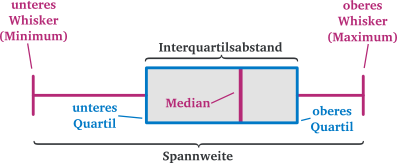
\includegraphics[width=0.45\textwidth]{includes/figures/definition_boxplot.png}
        \end{center}
    \end{wrapfigure}
    Der \emph{Box-Plot} ist ein Diagramm, das zur grafischen Darstellung der Verteilung eines mindestens ordinalskalierten Merkmals verwendet wird.

    Es fasst dabei verschiedene robuste Streuungs- und Lagemaße in einer Darstellung zusammen.

    Ein Box-Plot soll schnell einen Eindruck darüber vermitteln, in welchem Bereich die Daten liegen und wie sie sich über diesen Bereich verteilen. Deshalb werden alle Werte der sogenannten Fünf-Punkte-Zusammenfassung, also der Median, die zwei Quartile und die beiden Extremwerte, dargestellt.

    Zusammengefasst lassen sich folgende Kennwerte ablesen:

    \begin{center}
        \begin{tabular}{|l|p{0.4\linewidth}|p{0.3\linewidth}|}
            \hline
            Kennwert        & Beschreibung                                                                          & Lage im Box-Plot                                   \\
            \hline
            \hline
            Minimum         & Kleinster Datenwert des Datensatzes                                                   & Ende eines Whiskers oder entferntester Ausreißer   \\
            \hline
            Unteres Quartil & Die kleinsten 25\% der Datenwerte sind kleiner als dieser oder gleich diesem Kennwert & Beginn der Box                                     \\
            \hline
            Oberes Quartil  & Die kleinsten 75\% der Datenwerte sind kleiner als dieser oder gleich diesem Kennwert & Ende der Box                                       \\
            \hline
            Maximum         & Größter Datenwert des Datensatzes                                                     & Ende eines Whiskers oder entferntester Ausreißer   \\
            \hline
            Spannweite      & Gesamter Wertebereich des Datensatzes                                                 & Länge des gesamten Box-Plots (inklusive Ausreißer) \\
            \hline
            Quartilsabstand & Wertebereich, in dem sich die mittleren 50\% der Daten befinden                       & Ausdehnung der Box                                 \\
            \hline
        \end{tabular}
    \end{center}
\end{defi}

\begin{defi}{Empirische Varianz}
    Die \emph{empirische Varianz} bzw. \emph{Stichprobenvarianz}  ist eine statistische Angabe für die Streubreite von Werten einer Stichprobe.

    Sie gehört zu den Streuungsmaßen und beschreibt die mittlere quadratische Abweichung der einzelnen Messwerte vom empirischen Mittelwert.

    Sie stellt damit eine Art durchschnittliches Abweichungsquadrat dar.

    Die positive Wurzel der empirischen Varianz ist die \emph{empirische Standardabweichung}.
    Die empirische Standardabweichung stellt das gebräuchlichste Streuungsmaß dar.

    Es gilt:
    \begin{itemize}
        \item Für Stichproben in einer Urliste, wobei $x_i$ die Ausprägung des $i$-ten Elements darstellt:
              \[
                  s^2 = \frac{1}{n-1} \sum_{i=1}^{n} (x_i - \conj{x})^2 = \frac{1}{n-1} \left( \sum_{i=1}^{n} x_i^2 - n\cdot \conj{x}^2 \right)
              \]
        \item Für eine unklassierte Häufigkeitstabelle, wobei $n_j$ die absolute Häufigkeit des $j$-ten Elements $a_j$ darstellt:
              \[
                  s^2 = \frac{1}{n-1} \sum_{j=1}^{m} (a_j - \conj{x})^2 \cdot n_j = \frac{1}{n-1} \left( \sum_{j=1}^{m} a_j^2 \cdot n_j - \conj{x}^2 \right)
              \]
        \item Für eine klassierte Häufigkeitstabelle, wobei $n_j$ die absolute Häufigkeit der $j$-ten Klasse $A_j$, und $\alpha_j$ die Klassenmitte darstellt:
              \[
                  s^2 \approx \frac{1}{n-1} \sum_{j=1}^{m} \alpha_j^2 \cdot n_j - \frac{1}{n(n-1)} \left( \sum_{j=1}^{m} \alpha_j \cdot n_j \right)^2
              \]
    \end{itemize}

    Insgesamt gilt natürlich jeweils für die empirische Standardabweichung:
    \[
        s = \sqrt{s^2}
    \]
\end{defi}

\begin{defi}{Variationskoeffizient}
    Die Motivation für den \emph{Variationskoeffizienten} ist, dass eine statistische Variable mit großem Mittelwert bzw. eine Zufallsvariable mit großem Erwartungswert im Allgemeinen eine größere Varianz aufweist als eine mit einem kleinen Mittel- bzw. Erwartungswert.

    Da die Varianz und die daraus abgeleitete Standardabweichung nicht normiert sind, kann ohne Kenntnis des Mittelwerts nicht beurteilt werden, ob eine Varianz groß oder klein ist.

    Der Variationskoeffizient ist eine Normierung der Varianz: Ist die Standardabweichung größer als der Mittelwert bzw. der Erwartungswert, so ist der Variationskoeffizient größer 1.

    Es gilt:
    \[
        \VarK = \frac{s}{\conj{x}}
    \]
\end{defi}

\subsection{Lineare Regression und Korrelation}

\begin{defi}{Empirische Kovarianz}
    Die \emph{empirische Kovarianz} bzw. \emph{Stichprobenkovarianz} ist  eine nichtstandardisierte Maßzahl für den (linearen) Zusammenhang zweier statistischer Variablen.

    Ist die Kovarianz positiv, dann gehen kleine Werte der einen Variable überwiegend einher mit kleinen Werten der anderen Variable und gleichfalls für große Werte.
    Für eine negative Kovarianz ist das genau umgekehrt.

    Es werden benötigt:
    \begin{itemize}
        \item Empirische Varianzen der beiden Variablen $X$ und $Y$
              \begin{itemize}
                  \item $s_x^2$ und $s_y^2$
              \end{itemize}
        \item Arithmetische Mittelwerte der beiden Variablen $X$ und $Y$
              \begin{itemize}
                  \item $\conj{x}$ und $\conj{y}$
              \end{itemize}
    \end{itemize}

    Es gilt:
    \[
        \Cov(X, Y) = s_{x, y} = \frac{1}{n-1} \sum_{i=1}^{n} (x_i - \conj{x}) (y_i - \conj{y}) = \frac{1}{n-1} \left( \sum_{i=1}^{n} x_i y_i - n\cdot \conj{x} \cdot \conj{y} \right)
    \]
\end{defi}

\begin{defi}{Korrelationskoeffizient (empirisch)}
    Die Größe der Kovarianz lässt sich nicht sinnvoll interpretieren.

    Der \emph{empirische Korrelationskoeffizient} ist ein Maß für den Grad des linearen Zusammenhangs zwischen zwei Merkmalen, das nicht von den Maßeinheiten der Messung abhängt und somit dimensionslos ist.

    Er kann Werte zwischen $-1$ und $+1$ annehmen.
    Bei einem Wert von $+1$ (bzw. $-1$) besteht ein vollständig positiver (bzw. negativer) linearer Zusammenhang zwischen den betrachteten Merkmalen.

    Wenn der Korrelationskoeffizient den Wert $0$ aufweist, hängen die beiden Merkmale überhaupt nicht linear voneinander ab.
    Allerdings können diese ungeachtet dessen in nichtlinearer Weise voneinander abhängen.

    Es gilt:
    \[
        r_{x, y} = \frac{s_{x, y}}{s_x \cdot s_y} = \frac{\sum_{i=1}^{n} (x_i - \conj{x}) (y_i - \conj{y})}{\sqrt{ \sum_{i=1}^{n} (x_i - \conj{x})^2 } \cdot \sqrt{ \sum_{i=1}^{n} (y_i - \conj{y})^2 }}
    \]

    Klärung beliebter Missverständnisse:
    \begin{itemize}
        \item $r_{x, y}$ sagt nichts über die Größe der Geradensteigung aus.
        \item $r_{x, y} = 0$ bedeutet nur, dass zwischen $X$ und $Y$ kein \emph{linearer} Zusammenhang besteht.
        \item $r_{x, y}$ nahe bei $\pm 1$ bedeutet keinen kausalen Zusammenhang.
        \item $r_{x, y}$ gilt nur für quantitative Merkmale.
    \end{itemize}
\end{defi}

\begin{defi}{Bestimmtheitsmaß}
    Das \emph{Bestimmtheitsmaß} bewertet als Quadrat des Korrelationskoeffizienten die Anpassungsgüte der zu einem Datensatz ermittelten Regressionsgerade und hat einen Wert zwischen $0$ und $1$, wobei der Wert $1$ die Situation beschreibt, dass alle Datenpaare auf einer Geraden liegen und damit perfekte Anpassung vorliegt.

    Es gilt:
    \[
        B_{x, y} = r_{x, y}^2
    \]
\end{defi}

\begin{defi}{Lineare Regression}
    Das Ziel einer \emph{Regression} ist es, eine abhängige Variable durch eine oder mehrere unabhängige Variablen zu erklären.

    Bei der \emph{einfachen linearen Regression} wird eine abhängige Variable durch lediglich eine unabhängige Variable erklärt.

    Das Modell der linearen Einfachregression geht daher von zwei metrischen Größen aus:
    \begin{itemize}
        \item einer Einflussgröße $X$ (auch: erklärende Variable, Regressor oder unabhängige Variable)
        \item einer Zielgröße $Y$ (auch: abhängige Variable, erklärte Variable oder Regressand)
    \end{itemize}

    Des Weiteren liegen $n$ Paare $(x_1, y_1), \ldots, (x_n, y_n)$ von Messwerten vor, die in einem funktionalen Zusammenhang stehen:\footnote{Diese werden meist als Streudiagramm dargestellt.}
    \[
        Y_i = \underbrace{f(x_i; \hat{a}, \hat{b}, \ldots)}_{\text{systematische Komponente}} + \underbrace{\epsilon_i}_{\text{stochastische Komponente}}
    \]

    Die stochastische Komponente beschreibt nur noch zufällige Einflüsse (z. B. zufällige Abweichungen wie Messfehler), alle systematischen Einflüsse sind in der systematischen Komponente enthalten.

    Die lineare Einfachregression stellt den Zusammenhang zwischen der Einfluss- und der Zielgröße mithilfe von zwei festen, unbekannten, reellen Parametern $\hat{a}$ und $\hat{b}$ auf lineare Weise her.

    Die Regressionsfunktion ist wie folgt definiert:
    \[
        f(x_i; \hat{a}, \hat{b}) = \hat{a} + \hat{b} x_i
    \]

    Wir schätzen mithilfe der Methode der kleinsten Quadrate und erhalten als Regressionsparameter $\hat{a}$ und $\hat{b}$:
    \[
        \hat{b} = \frac{s_{x,y}}{s_x^2} = \frac{\sum_{i=1}^{n} (x_i - \conj{x}) (y_i - \conj{y})}{\sum_{i=1}^{n} (x_i - \conj{x})^2}
    \]
    \[
        \hat{a} = \conj{y} - \hat{b} \conj{x}
    \]

    Damit erhalten wir die Regressionsgerade:\footnote{Für jeden Wert $x_i$ können damit die Störgrößen bzw. Residuen berechnet werden mit $\hat{\epsilon}_i = y_i - \hat{y}_i$.}
    \[
        \hat{y}_i = \hat{a} + \hat{b} x_i
    \]
\end{defi}

\begin{example}{Lineare Regression (empirische Kovarianz)}
    Die Schülerinnen und Schüler wurden vor der Klausur anonym befragt, wie viele Stunden Schlaf sie vor der Klausur gehabt haben:
    \begin{center}
        \begin{tabular}{|c||C|C|C|C|C|C|C|C|C|C|}
            \hline
            Note   & 2 & 4 & 3 & 5 & 6 & 6 & 1 & 2 & 5 & 4 \\
            \hline
            Schlaf & 9 & 5 & 6 & 5 & 1 & 2 & 9 & 8 & 4 & 7 \\
            \hline
        \end{tabular}
    \end{center}

    Berechnen Sie aus den Daten:
    \begin{enumerate}[\alph*)]
        \item die empirische Kovarianz
        \item den empirischen Korrelationskoeffizient
        \item die lineare Regression
    \end{enumerate}

    Erstellen Sie ein Streudiagramm und zeichnen Sie die Regressionsgerade ein.

    \exampleseparator

    a) Es gilt:
    \[
        \Cov(X, Y) = s_{XY} = \frac{1}{n-1} \cdot \sum_{i=1}^{n} (x_i - \conj{x})(y_i - \conj{y}) = \frac{1}{n-1} \left( \sum_{i=1}^{n} x_iy_i - n \cdot \conj{x} \cdot \conj{y} \right)
    \]

    Wir berechnen zuerst die arithmetischen Mittel von $X$ und $Y$ wie folgt:
    \[
        \conj{x} = \frac{1}{n} \sum_{i=1}^n x_i = \frac{1}{10} \cdot (2 + 4 + 3 + 5 + 6 + 6 + 1 + 2 + 5 + 4) = \frac{19}{5} = 3.8
    \]
    \[
        \conj{y} = \frac{1}{n} \sum_{i=1}^n y_i = \frac{1}{10} \cdot (9 + 5 + 6 + 5 + 1 + 2 + 9 + 8 + 4 + 7) = \frac{28}{5} = 5.6
    \]

    Damit gilt:
    \begin{alignat*}{1}
        \Cov(X, Y) = s_{xy} & = \frac{1}{n-1} \cdot \sum_{i=1}^{n} (x_i - \conj{x})(y_i - \conj{y})                         \\
                            & = \frac{1}{n-1} \left( \sum_{i=1}^{n} x_iy_i - n \cdot \conj{x} \cdot \conj{y} \right)        \\
                            & = \frac{1}{9} \left( \sum_{i=1}^{n} x_iy_i - 10 \cdot \frac{19}{5} \cdot \frac{28}{5} \right) \\
                            & = \frac{1}{9} \left( \sum_{i=1}^{n} x_iy_i - \frac{1064}{5} \right)                           \\
                            & = \frac{1}{9} \sum_{i=1}^{n} x_iy_i - \frac{1064}{45}                                         \\
                            & = \frac{1}{9} \cdot 172 - \frac{1064}{45}                                                     \\
                            & = -\frac{68}{15} \approx -4.53
    \end{alignat*}
\end{example}

\begin{example}{Lineare Regression (empirischer Korrelationskoeffizient)}
    b) Es gilt:
    \[
        r_{xy} = \frac{s_{xy}}{s_x \cdot s_y} = \frac{\sum_{i=1}^{n} (x_i - \conj{x})(y_i - \conj{y})}{\sqrt{\sum_{i=1}^{n} (x_i - \conj{x})^2 \cdot \sum_{i=1}^{n} (y_i - \conj{y})^2 }}
    \]
    Wir berechnen zuerst die empirischen Standardabweichungen $s_x$ und $s_y$ wie folgt:
    \[
        s_x^2 = \frac{1}{n-1} \sum_{i=1}^{n} (x_i - \conj{x})^2 = \frac{1}{9} \sum_{i=1}^{n} \left(x_i - \frac{19}{5} \right)^2 = \frac{46}{15} \implies s_x = \sqrt{\frac{46}{15}} = \frac{\sqrt{690}}{15}
    \]
    \[
        s_y^2 = \frac{1}{n-1} \sum_{i=1}^{n} (y_i - \conj{y})^2 = \frac{1}{9} \sum_{i=1}^{n} \left(y_i - \frac{28}{5} \right)^2 = \frac{38}{5} \implies s_y = \sqrt{\frac{38}{5}} = \frac{\sqrt{190}}{5}
    \]

    Damit gilt dann:
    \[
        r_{xy} = \frac{s_{xy}}{s_x \cdot s_y} = \frac{-\nicefrac{68}{15}}{\nicefrac{\sqrt{690}}{15} \cdot \nicefrac{\sqrt{190}}{5}} = - \frac{34\sqrt{1311}}{1311} \approx -0.93903
    \]
\end{example}

\begin{example}{Lineare Regression (empirischer Korrelationskoeffizient)}
    c) Die Regressionsgerade ist gegeben mit:
    \[
        \hat{y}_i = \hat{a} + \hat{b}x_i
    \]

    Es gilt:
    \[
        \hat{b} = \frac{s_{xy}}{s_x^2} = \frac{-\nicefrac{68}{15}}{\nicefrac{46}{15}} = - \frac{34}{23} \approx -1.478
    \]
    \[
        \hat{a} = \conj{y} - \hat{b} \cdot \conj{x} = \frac{28}{5} + \frac{34}{23} \cdot \frac{19}{5} = \frac{258}{23} \approx 11.217
    \]

    Und damit erhalten wir:
    \[
        \hat{y}_i = 11.217 -1.478x_i
    \]
\end{example}

\begin{example}{Lineare Regression (Regressionsgerade)}
    \begin{center}
        \begin{tikzpicture}
            \begin{axis}[%
                    scale only axis,
                    width=0.7\textwidth,
                    height=0.2\textheight,
                    grid=both,
                    xlabel={Note},
                    ylabel={Schlaf in Stunden},
                    scatter/classes={%
                            a={mark=o,draw=black}}]
                \addplot[scatter,only marks,%
                    scatter src=explicit symbolic]%
                table {
                        x y
                        2 9
                        4 5
                        3 6
                        5 5
                        6 1
                        6 2
                        1 9
                        2 8
                        5 4
                        4 7
                    };
                \addplot[domain=1:6, color=blue]{11.217 -1.478 * x};
            \end{axis}
        \end{tikzpicture}
    \end{center}
\end{example}